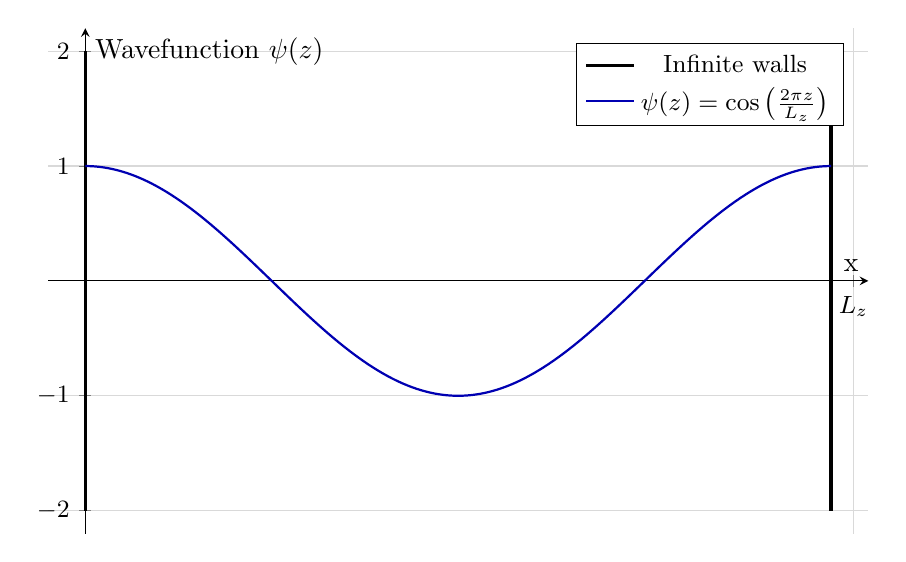
\begin{tikzpicture}
  \begin{axis}[
      xlabel={x},
      ylabel={Wavefunction $\psi(z)$},
      xmin=-0.05, xmax=1.05,
      ymin=-2.2, ymax=2.2,
      grid=major,
      grid style={gray!30},
      axis lines=middle,
      width=12cm,
      height=8cm,
      xtick={0, 1.03},
      xticklabels={0, $L_z$},
      xticklabel style={font=\small},
      yticklabel style={font=\small},
      legend pos=north east,
      legend style={font=\small}
    ]
    % Infinite potential walls (vertical lines)
    \addplot[black, very thick, domain=-0.2:2, samples=2] {-2.5}; %
    \addlegendentry{Infinite walls}
    \draw[black, very thick] (axis cs:0,-2) -- (axis cs:0,2);
    \draw[black, very thick] (axis cs:1,-2) -- (axis cs:1,2);

    % Wavefunction psi_7(z) = sin(7*pi*z/L_z)
    % For L_z = 1, this becomes sin(7*pi*z)
    \addplot[
      domain=0:1,
      samples=400,
      thick,
      blue!70!black
    ] {cos(deg(2*pi*x))};

    % Add legend entry
    \addlegendentry{$\psi(z) = \cos\left(\frac{2\pi z}{L_z}\right)$}

    % Add wall labels
    \node[black, above] at (axis cs:-0.1,1.8) {\small Wall};
    \node[black, above] at (axis cs:-0.1,1.8) {\small Wall};
  \end{axis}
\end{tikzpicture}
